\documentclass{minimal}
\usepackage{tikz}
\usepackage{amsmath}
\usepackage{amsfonts}
\usepackage{amssymb}
\usepackage{graphicx}

\usetikzlibrary{positioning,arrows}
\usetikzlibrary{decorations.pathmorphing}
\usetikzlibrary{decorations.markings}
\usetikzlibrary{arrows,snakes,shapes}

\tikzset{
TT/.style={decorate, draw=black,
    decoration={coil,aspect=0.7,segment length=3.2pt,amplitude=2pt}}
}
\tikzset{
sigma/.style={dashed}
}
\tikzset{
arb1/.style={dashed}
}
\tikzset{
arb2/.style={decorate, decoration={snake}}
}


\begin{document}
\scalebox{0.75}{
\begin{equation*}
  \boxed{
\mbox{\fontsize{19.28}{21.6}\selectfont\( %
\partial_t
\left(
  \hspace{-10pt}
  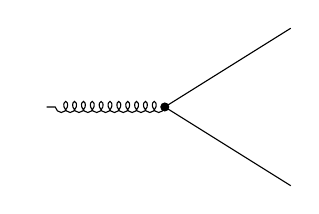
\begin{tikzpicture}[>=stealth,scale=1.00,baseline=-0.1cm]
    \draw[TT] (-1,0) -- (-2.5,0) node[anchor=east] {};
    \draw (-1,0) -- (.6,1);
    \draw (-1,0) -- (.6,-1);
    \draw[fill] (-1,0) circle [radius=0.05];
  \end{tikzpicture}
  \hspace{10pt}
\right)
=
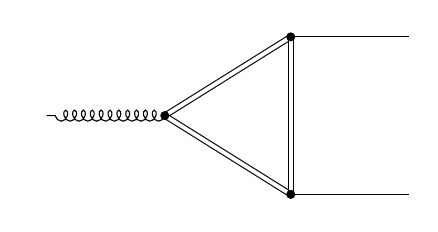
\begin{tikzpicture}[>=stealth,scale=1.00,baseline=-0.1cm]
\draw[TT] (-1,0) -- (-2.5,0) node[anchor=east] {};
\draw (.6,-1) -- (2.1,-1) node[anchor=east] {};
\draw (.6,1) -- (2.1,1) node[anchor=east] {};

\draw[double,double distance=.5mm] (-1,0) -- (.6,1);
\draw[double,double distance=.5mm] (-1,0) -- (.6,-1);
\draw[double,double distance=.5mm] (.6,1) -- (.6,-1);


\draw[fill] (-1,0) circle [radius=0.05];
\draw[fill] (.6,1) circle [radius=0.05];
\draw[fill] (.6,-1) circle [radius=0.05];
\end{tikzpicture}
+
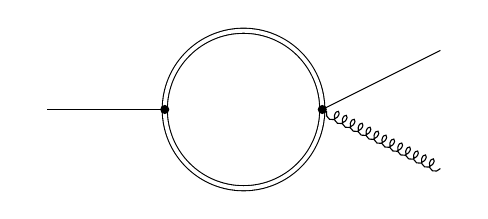
\begin{tikzpicture}[>=stealth,scale=1.00,baseline=-0.1cm]
\draw (2.5,0.75) node[anchor=west] {} -- (1,0);
\draw[TT] (2.5,-0.75) node[anchor=west] {} -- (1,0);
\draw (-1,0) -- (-2.5,0) node[anchor=east] {};

\draw[double,double distance=.5mm] (-1,0) arc (180:0:1cm);
\draw[double,double distance=.5mm] (-1,0) arc (180:360:1cm);

\draw[fill] (-1,0) circle [radius=0.05];
\draw[fill] (1,0) circle [radius=0.05];
\end{tikzpicture}
+
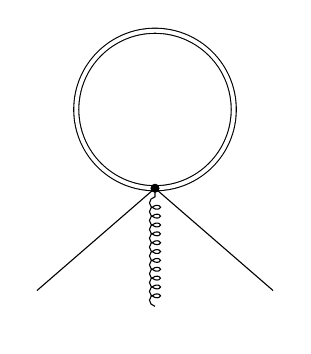
\begin{tikzpicture}[>=stealth,scale=1,baseline=-0.1cm]
\draw (-1.5,-2.3) node[anchor=north] {} -- (0,-1);
\draw[TT] (0,-2.5) node[anchor=north] {} -- (0,-1);
\draw (1.5,-2.3) node[anchor=north] {} -- (0,-1);

\draw (0,-1)[double,double distance=.5mm] arc (270:-90:1cm);

\draw[fill] (0,-1) circle [radius=0.05];
\end{tikzpicture}
+
\,\cdots
\)}
}
\end{equation*}
}
\end{document}
